\subsection{MSVC: SYSTEMTIME example}
\label{sec:SYSTEMTIME}

\newcommand{\FNSYSTEMTIME}{\footnote{\href{http://go.yurichev.com/17260}{MSDN: SYSTEMTIME structure}}}

Let's take the SYSTEMTIME\FNSYSTEMTIME{} win32 structure that describes time.

This is how it's defined:

\begin{lstlisting}[caption=WinBase.h]
typedef struct _SYSTEMTIME {
  WORD wYear;
  WORD wMonth;
  WORD wDayOfWeek;
  WORD wDay;
  WORD wHour;
  WORD wMinute;
  WORD wSecond;
  WORD wMilliseconds;
} SYSTEMTIME, *PSYSTEMTIME;
\end{lstlisting}

Let's write a C function to get the current time:

\lstinputlisting{patterns/15_structs/1_systemtime/systemtime.c}

We get (MSVC 2010):

\lstinputlisting[caption=MSVC 2010 /GS-]{patterns/15_structs/1_systemtime/systemtime.asm}

16 bytes are allocated for this structure in the local stack~---that is exactly \TT{sizeof(WORD)*8}
(there are 8 WORD variables in the structure).

\newcommand{\FNMSDNGST}{\footnote{\href{http://go.yurichev.com/17261}{MSDN: GetSystemTime function}}}

Pay attention to the fact that the structure begins with the \TT{wYear} field.
It can be said that a pointer to the SYSTEMTIME structure is passed to the \TT{GetSystemTime()}\FNSYSTEMTIME,
but it is also can be said that a pointer to the \TT{wYear} field is passed, and that is the same!
\TT{GetSystemTime()} writes the current year to the WORD pointer pointing to, then shifts 2 bytes
ahead, writes current month, etc., etc.

\clearpage
\subsection{\olly}
\myindex{\olly}

Let's compile this example in MSVC 2010 with \TT{/GS- /MD} keys and run it in \olly.

Let's open windows for data and stack at the address which is passed as the first argument of the
\TT{GetSystemTime()} function, and let's wait until it's executed. We see this:

\begin{figure}[H]
\centering
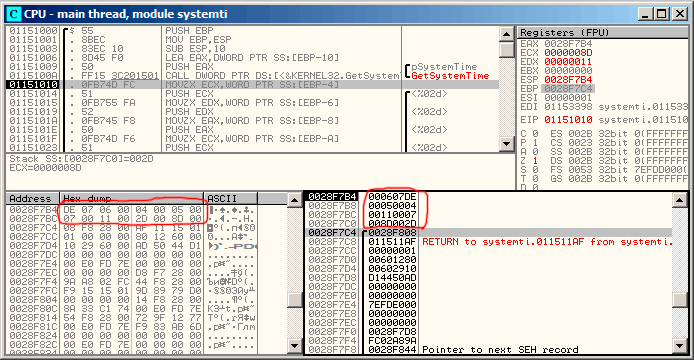
\includegraphics[scale=\FigScale]{patterns/15_structs/1_systemtime/olly_systemtime1.png}
\caption{\olly: \TT{GetSystemTime()} just executed}
\label{fig:struct_olly_1}
\end{figure}

The system time of the function execution on my computer is 9 december 2014, 22:29:52:

\begin{figure}[H]
\centering
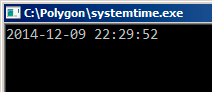
\includegraphics[scale=\NormalScale]{patterns/15_structs/1_systemtime/olly_systemtime2.png}
\caption{\olly: \printf output}
\label{fig:struct_olly_2}
\end{figure}

So we see these 16 bytes in the
data window: 
\begin{lstlisting}
DE 07 0C 00 02 00 09 00 16 00 1D 00 34 00 D4 03
\end{lstlisting}

Each two bytes represent one field of the structure. 
Since the \gls{endianness} is \IT{little endian}, 
we see the low byte first and then the high one.

Hence, these are the values currently stored in memory:

\begin{center}
\begin{tabular}{ | l | l | l | }
\hline
\headercolor{} Hexadecimal number & 
\headercolor{} decimal number & 
\headercolor{} field name \\
\hline
0x07DE & 2014	& wYear \\
\hline
0x000C & 12	& wMonth \\
\hline
0x0002 & 2	& wDayOfWeek \\
\hline
0x0009 & 9	& wDay \\
\hline
0x0016 & 22	& wHour \\
\hline
0x001D & 29	& wMinute \\
\hline
0x0034 & 52	& wSecond \\
\hline	
0x03D4 & 980	& wMilliseconds \\
\hline
\end{tabular}
\end{center}

The same values are seen in the stack window, but they are grouped as 32-bit values.

And then \printf just takes the values it needs and outputs them to the console.

Some values aren't output by \printf  (\TT{wDayOfWeek} and \TT{wMilliseconds}), 
but they are in memory right now, available for use.



\subsubsection{Replacing the structure with array}

The fact that the structure fields are just variables located side-by-side, can be easily demonstrated by doing the following.
Keeping in mind the \TT{SYSTEMTIME} structure description, it's possible to rewrite this simple example like this:

\lstinputlisting{patterns/15_structs/1_systemtime/systemtime2.c}

The compiler grumbles a bit:

\begin{lstlisting}
systemtime2.c(7) : warning C4133: 'function' : incompatible types - from 'WORD [8]' to 'LPSYSTEMTIME'
\end{lstlisting}

But nevertheless, it produces this code:

\lstinputlisting[caption=\NonOptimizing MSVC 2010]{patterns/15_structs/1_systemtime/systemtime2.asm}

And it works just as the same!

It is very interesting that the
result in assembly form cannot be distinguished from the result of the previous compilation.

So by looking at this code, one cannot say for sure if there was a structure declared, or an array. 

Nevertheless, no sane person would do it, as it is not convenient. 

Also the structure fields may be changed by developers, swapped, etc.

We will not study this example in \olly, because it will be just the same as in the case with the structure.

